  \section{Project}
A smart home system has many features that can make life easier. For example, consider a smart heating and cooling system in which the heater and air conditioner can be easily adjusted via smartphone. A smart door, smart alarm, and smart light system are also examples of smart house systems. However, in our project, we will only demonstrate how the smart light system works in the smart home system.

Smartphones are the friendly gadgets which have made everything reachable through a touch. They have occupied such a huge place in our daily lives that it is no wonder that for most of us, a smartphone is the first thing we look at in the morning and it is the last thing we see before going to bed. They are the new craze and we cannot deny that they have made life easier than ever. They are portable and easy to carry around and we always carry them with us anytime and anywhere we go, for example in our pockets. This convenience and portability of smartphones have led the marketers and the designers to take the opportunity to use these advantages into developing services and solutions around the mobile domain, mainly by creating applications on mobile phones. For example, there are apps to shop online, do banking, trade stocks and uncountable day to day tasks. Then how can home automation systems remain isolated from mobile technology?
 
In this project, a home automation system is designed which can be controlled by any smartphone. The automation system connects with the smartphone through Bluetooth. The smartphone will then send control signals to switch home appliances ON or OFF by an android app through Bluetooth interface. An app named “Bluetooth Terminal” is used on the smartphone which is capable of sending text strings to a paired device. The app will pair with the home automation system through Bluetooth Low Energy Module by using ESP32.  
 
The Arduino board receives the user commands in the form of numbers from the smart phone through Bluetooth interface. These numbers are assigned to the home appliances and the appliances are toggled either ON or OFF on receiving the numeric command. The ESP32  sketch looks for the numeric commands from the Bluetooth module and operates relays to switch appliances.

\subsection{Diagrams}
To have a deeper understanding on our project, use case diagram is also being included. There are two actors in our use case diagram: the user and the server. The user will be able to control all of the system's features, including turning on and off LEDs, blinking LEDs, party mode, and night mode. In this system, the user must open the BLE apps in order to type the command, which will then produce output. Figure 1 show the use case diagram for smart light system. In this system, the server will communicate with the client, which in our case is a smartphone. In addition, the server will be able to display the output.


\begin{figure}[htp]
    \centering
    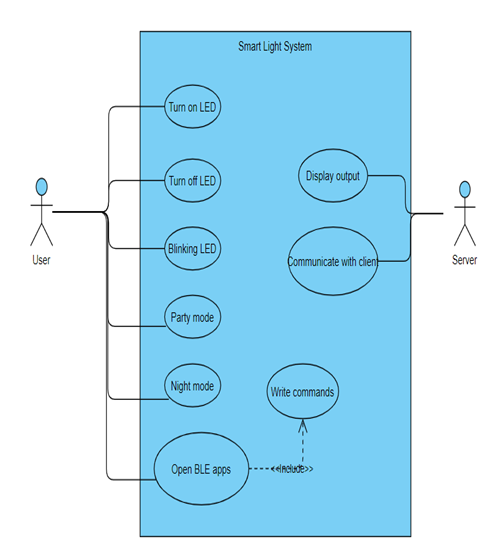
\includegraphics{imageusecase.png}
    \caption{Use Case Diagram}
    \label{bulat1}
\end{figure}



\subsection{Hardware}

A lot of hardware is required for our project. Each piece of hardware will serve a specific purpose in the creation of our project. The list of hardware required for our projects, as well as a description of its function in our project, is provided below.


\subsection{Features and List of commands}
The smartphone in our smart light system will communicate with the server via BLE protocol to control the features that have been implemented in our smart light system. Our smart lighting system's features are listed below. Some commands have been specified and inserted on the smartphone that is already connected to the ESP32 via BLE in order for our features to show their output. It means that different commands will produce different results. In addition, users must download specific apps, which will assist in connecting to EPS32 and inserting commands. Figure 1 depicts the apps we used to connect our smartphone to the ESP32. If you have an iPhone, you can easily find this app in the "Apple store." Figure 12 also shows where the command must be inserted in order to produce the desired output.

\begin{table}[]
\begin{center}
\caption{Features in Smart Light}
\begin{tabular}{|l|l|}
\hline
No & Smart   Light Features \\ \hline
2. & Turn on LED            \\ \hline
3. & Turn off LED           \\ \hline
4. & Turn on night mode     \\ \hline
5. & Turn on party mode     \\ \hline
6. & Change color           \\ \hline
7. & Play sound             \\ \hline
\end{tabular}
\end{center}
\end{table}



\begin{figure}[htbp]
\centerline{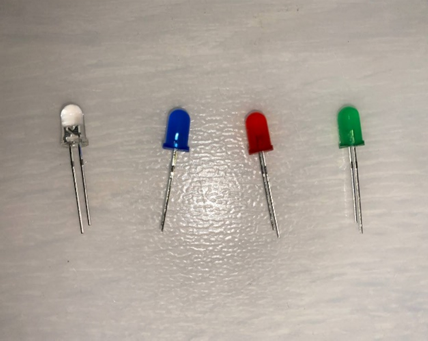
\includegraphics{image1.png}}
\caption{LED (white,blue,red,green)}
\label{fig}
\end{figure}

\begin{figure}[htbp]
\centerline{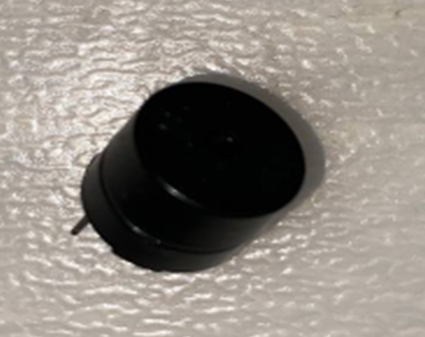
\includegraphics{image2.png}}
\caption{Buzzer}
\label{fig}
\end{figure}

\begin{figure}[htbp]
\centerline{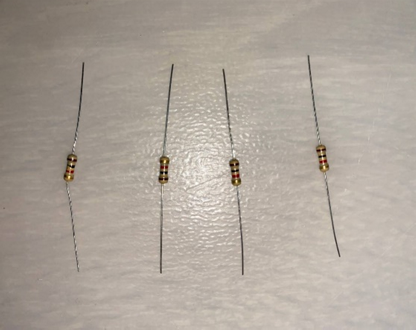
\includegraphics{image3.png}}
\caption{Resistors for 4 LED}
\label{fig}
\end{figure}

\begin{figure}[htbp]
\centerline{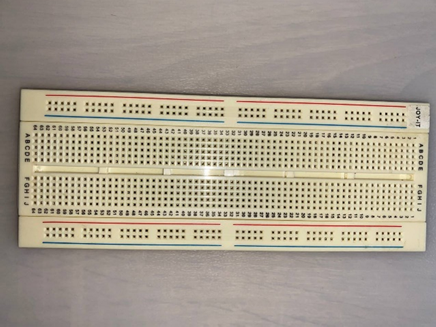
\includegraphics{image4.png}}
\caption{Breadboard}
\label{fig}
\end{figure}

\begin{figure}[htbp]
\centerline{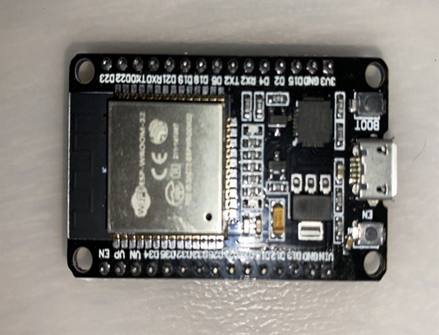
\includegraphics{image5.png}}
\caption{ESP32}
\label{fig}
\end{figure}



\subsection{Result}

We'll offer an example of our project's results in this documentation as well. Our smart lighting system has a lot of features, as previously indicated. Only the output from the commands to switch on, turn off, and change the brightness will be shown in this example. Figure 8,9,10 shows the example.


\begin{table}[]
\caption{List of hardware and its function}
\begin{center}
\begin{tabular}{|l|l|}
\hline
Hardware                                                                   & Functions                                                                                                                                                                  \\ \hline
\begin{tabular}[c]{@{}l@{}}LED   (red, blue\\ , green, white)\end{tabular} & \begin{tabular}[c]{@{}l@{}}1. Indicate turn off and turn on\\ 2. Indicate brightness\\ 3. Indicate blinking\\ 4. Indicate night mode\\ 5. Indicate event lamp\end{tabular} \\ \hline
Jumper wire                                                                & \begin{tabular}[c]{@{}l@{}}1. Connect between breadboard \\     and component\end{tabular}                                                                                 \\ \hline
ESP32                                                                      & \begin{tabular}[c]{@{}l@{}}1. Support BLE protocol\\ 2. Act as a server to communicate\\     with mobile phone\end{tabular}                                                \\ \hline
USB cable                                                                  & \begin{tabular}[c]{@{}l@{}}1. Connect between ESP32 and \\ laptop to upload the code\\ 2. Support transmission and receiving data\end{tabular}                             \\ \hline
Breadboard                                                                 & 1. Place to put the components                                                                                                                                             \\ \hline
Buzzer                                                                     & 1. Play sound                                                                                                                                                              \\ \hline
Resistor 100 ohm                                                           & 1. Act as resistance                                                                                                                                                       \\ \hline
\end{tabular}
\end{center}
\end{table}















\begin{table}[]
\begin{center}
\caption{Lists of commands}
\begin{tabular}{|l|l|}
\hline
List of Commands & Function             \\ \hline
ONW              & Turn on white LED    \\ \hline
ONR              & Turn on red LED      \\ \hline
ONB              & Turn on blue LED     \\ \hline
ONG              & Turn on green LED    \\ \hline
OFFW             & Turn off white LED   \\ \hline
OFFR             & Turn off red LED     \\ \hline
OFFB             & Turn off blue LED    \\ \hline
OFFG             & Turn off green LED   \\ \hline
BLW              & Blinking white LED   \\ \hline
BLR              & Blinking red LED     \\ \hline
BLB              & Blinking blue LED    \\ \hline
BLG              & Blinking green LED   \\ \hline
NMW              & Night mode white LED \\ \hline
NMR              & Night mode red LED   \\ \hline
NMB              & Night mode blue LED  \\ \hline
NMG              & Night mode green LED \\ \hline
PARTY            & Party mode           \\ \hline
\end{tabular}
\end{center}
\end{table}


\begin{figure}[htbp]
\centerline{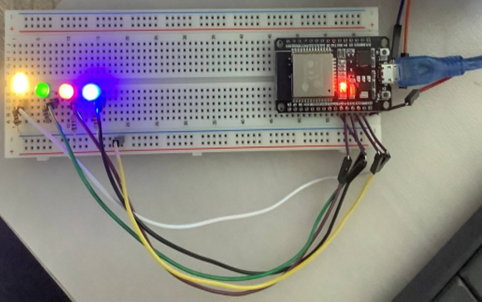
\includegraphics{image7.png}}
\caption{White, Green , Blue  and Red is turned on by using commands ONW,ONG,ONB,ONR respectively}
\label{fig}
\end{figure}




\begin{figure}[htbp]
\centerline{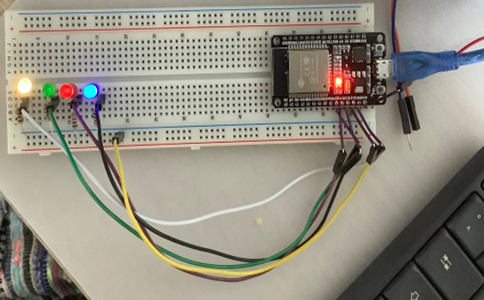
\includegraphics{image8.png}}
\caption{White, Green , Blue  and Red is in night mode by using commands NMW,NMG,NMB,NMR respectively}
\label{fig}
\end{figure}


\begin{figure}[htbp]
\centerline{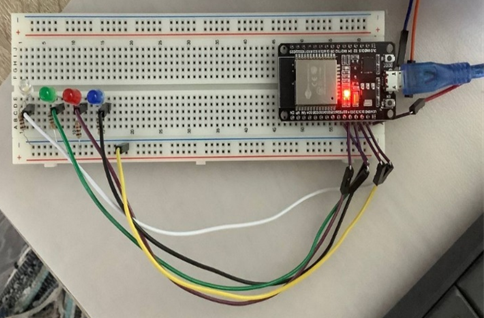
\includegraphics{image9.png}}
\caption{White, Green , Blue  and Red is turned off by using commands OFFW,OFFG,OFFB,OFFR respectively}
\label{fig}
\end{figure}



\begin{figure}[htbp]
\centerline{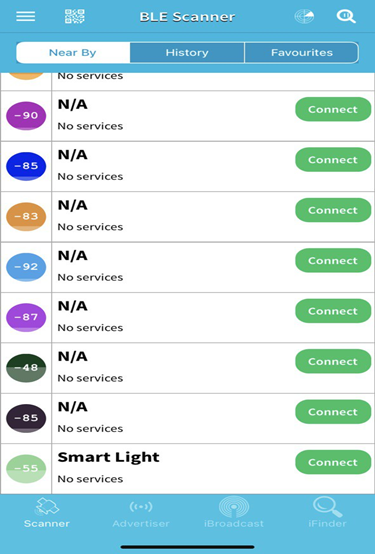
\includegraphics{image10.png}}
\caption{Apps that been used to connect with ESP32}
\label{fig}
\end{figure}




\begin{figure}[htbp]
\centerline{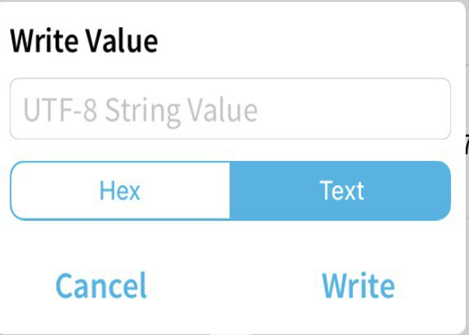
\includegraphics{image11.png}}
\caption{Place to put commands}
\label{fig}
\end{figure}








